%Tex spell check = en-US

\documentclass[12pt,a4paper]{article}
\usepackage{graphicx}
\usepackage{caption}
\usepackage{subcaption}
\usepackage[english]{varioref}
\usepackage[english]{babel}
\usepackage{datetime}
\usepackage{amsmath}
\usepackage{booktabs}
\usepackage{placeins}
\usepackage{url}
\usepackage{csquotes}
\usepackage{adjustbox}
\usepackage{listings}
\usepackage{float}
\usepackage{minted}
\usepackage{enumitem}
\usepackage{varwidth}
\usepackage[multiple]{footmisc}


\newlength{\storeparskip}
\setlength{\storeparskip}{\parskip}

\setlength{\parskip}{\baselineskip}%
\setlength{\parindent}{0pt}%


%-------------------- VARS ----------------------
\newcommand{\authorName}{Gilles Callebaut}
\newcommand{\dateSessionOne}{22/02/2019 13u30\ -\ 16u30}
\newcommand{\dateSessionTwo}{08/03/2019 13u30\ -\ 16u30}
\newcommand{\dateSessionThree}{22/03/2019 13u30\ -\ 16u30}
\newcommand{\softDeadline}{04/04/2019}
\newcommand{\hardDeadline}{11/04/2019}

\title{Lab Assignment --\ Data Transmission\\\vspace{0.5cm}{\Large Multimedia Networks}}
\author{\authorName}

\begin{document}

\maketitle
\vfill


\begin{center}

  \begin{minipage}{0.65\linewidth}
\begin{description}[style=multiline, leftmargin=4cm]
	\item[Lab session 1] \dateSessionOne
	\item[Lab session 2] \dateSessionTwo
	\item[Lab session 3] \dateSessionThree
\end{description}
\vfill
\begin{description}[style=multiline, leftmargin=4cm]
	\item[Soft deadline] \softDeadline
	\item[Hard deadline] \hardDeadline
\end{description}
\end{minipage}
\end{center}

\vfill
\clearpage

\section{Introduction}
Claude Shannon, an engineer at Bell Telephone Laboratories, and Warren Weaver sought to identify the quickest and most efficient way to get a message from one point to another. As a result of their studies, they developed their model of communication.

In these \textbf{three lab sessions} you are going to simulate a \textbf{communication model} as presented in Figure~\vref{fig:labo1multimedianetwerkendatatransmissiediagram}. This model is a simplified version of the Shannon-Weaver model of communication. The model will be implemented via \textbf{MATLAB}\footnote{Install the necessary toolboxes as described in Section~\ref{ap:sec:toolboxes}.} or \textbf{Python} (prefered).

\begin{figure}[h]
	\centering
	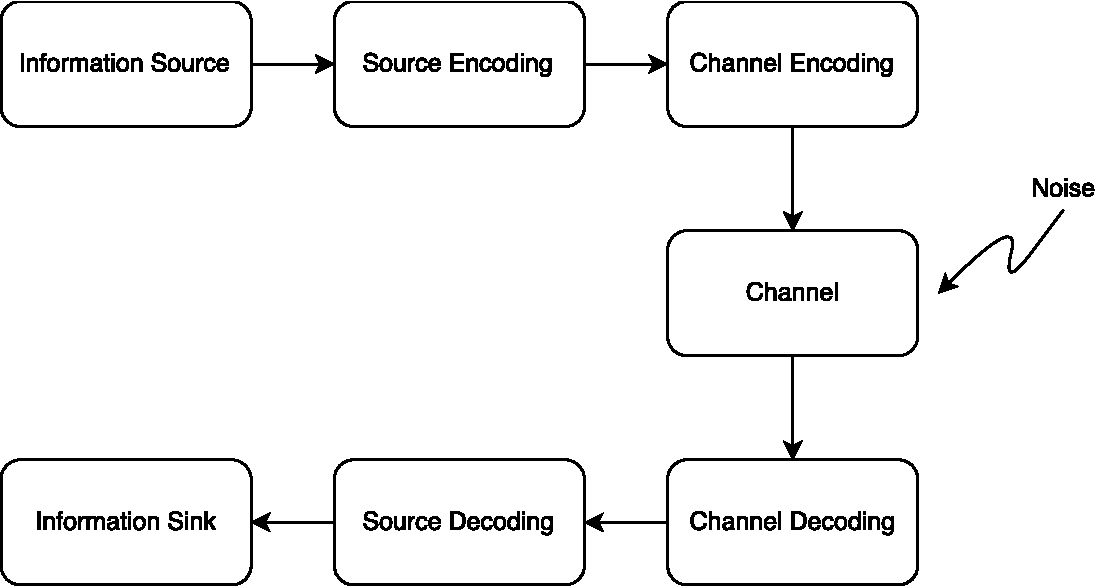
\includegraphics[width=0.7\linewidth]{labo_1_multimedianetwerken_datatransmissie_diagram}
	\caption{Simplified Model of Communication}\label{fig:labo1multimedianetwerkendatatransmissiediagram}
\end{figure}


\section{Communication Model}

Encoding and decoding data is computation intensive. Therefore, choosing a small image (e.g.,~40$\times$40) is strongly advised. To facilitate interoperability between the communication blocks, we suggest using a \textbf{bit stream} or a \textbf{byte stream} to \textbf{exchange} data between these blocks, i.e.\ every block will receive and send a bit or byte stream to the next one.

\subsection{Information Source}
An \textbf{image} will serve as the \textbf{information source}. 

\subsection{Source Encoding and Decoding}
Use \textbf{Huffman} and encoding as a \textbf{source encoding} mechanism.

\subsection{Channel Encoding and Decoding}
\textbf{Reed-Solomon} (RS) coding will be used for \textbf{channel encoding}. In this assignment modulation and channel characteristics can be neglected. The `transmitted' signal will be influenced by Additive white Gaussian noise (\textbf{AWGN}). Additionally, after applying Reed-Solomon encoding, the image can be altered through an image editor such as \textit{paint}. check if Reed-Solomon is able to resolve the introduced errors. 

A MATLAB template --and additional library functions-- can be found in the Appendix.
\textbf{TODO PYTHON}

\section{Objectives}
\begin{itemize}
	\item Build data transmission blocks via MATLAB or Python.%
	\item Experiment with the parameters such as the SNR or the code-word length of an RS message, and conclude.%
	\item Enable and disable blocks to determine their impact on the model.%
	\item Measure the transmitted bit stream size of each block and conclude.
	\item Measure the operation duration of each block and conclude.
	For instance, why is Huffman decoding slower than Huffman encoding?
	\item What is the correlation between entropy and the number of bits per symbol? (hint: Huffman)
	\item Calculate the number of resolved and unrecoverable errors after adding noise.
\end{itemize}

\section{Report}
Each student writes an \textbf{individual report}. This report must contain the \textbf{realization} of the aforementioned \textbf{objectives}. It must \textbf{demonstrate} that the student has \textbf{understood} the \textbf{communication model}. All MATLAB or Python \textbf{code} must be well \textbf{documented}.
The report has to be send to \texttt{gilles.callebaut@kuleuven.be} including the code. The code itself does not need to be included and discussed in the report.
The report is expected to be structured and styled as described in~\cite{hoogenboom2012write,kallestinova2011write}.

The report needs to be \textbf{submitted} before \hardDeadline, preferably before \softDeadline.

\cleardoublepage%
\appendix
\section{Template file}
\inputminted[linenos,tabsize=2,breaklines, fontsize=\footnotesize]{matlab}{../code/main.m}
\clearpage
\section{Library files}
\subsection{\texttt{convert\_to\_binary\_stream.m}}
\inputminted[linenos,tabsize=2,breaklines, fontsize=\footnotesize]{matlab}{../code/convert_to_binary_stream.m}
\subsection{\texttt{convert\_to\_dec\_stream.m}}
\inputminted[linenos,tabsize=2,breaklines, fontsize=\footnotesize]{matlab}{../code/convert_to_dec_stream.m}
\subsection{\texttt{print\_arrow.m}}
\inputminted[linenos,tabsize=2,breaklines, fontsize=\footnotesize]{matlab}{../code/print_arrow.m}
\clearpage
\subsection{\texttt{bit\_size.m}}
\inputminted[linenos,tabsize=2,breaklines, fontsize=\footnotesize]{matlab}{../code/bit_size.m}
\subsection{\texttt{gf2dec.m}}
\inputminted[linenos,tabsize=2,breaklines, fontsize=\footnotesize]{matlab}{../code/gf2dec.m}
\subsection{\texttt{decodeJpeg.m}}
\inputminted[linenos,tabsize=2,breaklines, fontsize=\footnotesize]{matlab}{../code/decodeJpeg.m}

\section{MATLAB Toolboxes}\label{ap:sec:toolboxes}
The following toolboxes should be installed:
\begin{itemize}
  \item \texttt{communication toolbox}
  %\item \texttt{data acq toolbox}
  \item \texttt{signal blocks}
\end{itemize}


\bibliographystyle{plain}
\bibliography{bib}
\end{document}
